\documentclass[letterpaper, preprint, paper,11pt]{AAS}	% for preprint proceedings
\usepackage{bm}
\usepackage{amsmath}
\usepackage{subfigure}
%\usepackage[notref,notcite]{showkeys}  % use this to temporarily show labels
\usepackage[colorlinks=true, pdfstartview=FitV, linkcolor=black, citecolor= black, urlcolor= black]{hyperref}
\usepackage{overcite}
\usepackage{footnpag}			      	% make footnote symbols restart on each page
\usepackage{listings}                   % Code Listings
\usepackage[table, x11names]{xcolor}                     % Code Coloring
% \usepackage[explicit]{titlesec}         % Paragraph Headers
% \usepackage{ulem}                       % Paragraph Headers Underlines
\usepackage{xfrac}                      % Slanted Fractions
\usepackage{booktabs}                   % Table Styling
\usepackage{multirow}                   % Table Styling

% CREATING PARAGRAPH HEADERS
% \titleformat{name=\paragraph,numberless}[runin]
    % {\normalfont\normalsize\bfseries}{}{15pt}{\uline{#1}}

% DEFINING CODE COLORS
\definecolor{comments}{rgb}{0.0, 0.5, 0.0}
\definecolor{keywords}{rgb}{0.01, 0.28, 1}

\lstset{
    basicstyle = \small\ttfamily,
    language = Python,
    frame = lines,
    backgroundcolor = \color{lightgray!10},
    commentstyle = \color{comments}\ttfamily\small,
    keywordstyle = \color{keywords}\bf\ttfamily\small,
    framesep=\fboxsep,
}


\PaperNumber{20-686}



\begin{document}

\title{Broad Trajectory Searches Using Monte Carlo Tree Search with the Inclusion of $\Delta$VEGA Trajectories}

\author{Burton A. Yale\thanks{Aerospace Engineering, Cal Poly Pomona, 3801 W Temple Ave., Pomona, California, 91786, USA} \thanks{Undergraduate Student, E-mail: bayale@cpp.edu},
\ Rohan D. Patel\footnotemark[1] \thanks{Undergraduate Student, E-mail: rohanpatel@cpp.edu},  
Jehosafat J. Cabrera\footnotemark[1] \thanks{Undergraduate Student, E-mail: jehosafatc@cpp.edu},
\ and Navid Nakhjiri\footnotemark[1] \thanks{Assistant Professor, E-mail: nnakhjiri@cpp.edu}
}

\maketitle{} 		


\begin{abstract}
Multiple flybys of the inner planets and the application of $V_{\infty}$ leveraging are essential trajectory design techniques to reduce the required launch energy for interplanetary missions. These trajectories are often difficult to formulate and require extensive computational resources. However, this problem can be classified as a sequential planning task which can be solved by a Monte Carlo Tree Search (MCTS) method. In this paper, a MCTS algorithm is developed and tested with a focus on reducing required $\Delta V$ from the spacecraft by introducing the concept of $\Delta V$EGA orbits. By performing deep space maneuvers to increase the energy from an Earth flyby, this algorithm will be able to find sequences previously not considered. Optimizations of several cases are studied to prove the feasibility of the tree search results. The algorithm will allow for inner-planetary flyby search planning for outer planetary missions.
\end{abstract}

\section{Introduction}
Broad trajectory searches are one of the first steps in mission planning, allowing for the selection of candidates given a list of constraints and a search space. As is the nature with combinatorial problems, every additional flyby adds another dimension to the search space. Brute force methods lead to expensive but thorough results. By pruning possible choices before the each selection, the overall computation time can be greatly decreased, at the expense of losing possible results. There have been various approaches to this method, from evolutionary/genetic algorithms, to particle swarm optimization, to enumerated searches, all with their own benefits and drawbacks. The method of interest for this paper is enumerated searches, a subset of grid searches, as recent work has proven their ability to quickly and accurately find multi-leg interplanetary trajectories\cite{Hennes2015}.

\textbf{M}onte \textbf{C}arlo \textbf{T}ree \textbf{S}earch (MCTS), is a heuristics-based adaptation of the enumerated search, and has the ability to both explore and exploit its environment. With this ability, it is possible for the algorithm to efficiently narrow down possible search paths for future iterations to explore further. As such, larger search spaces can be employed without exponential growth in computation time.

This algorithm will deliver a set of planetary sequences and the dates associated that meet mission criteria, such as destination, launch windows, total fuel budgets, etc. These results can then be passed on to the next phase of the design, optimization.


\section{Background}

Interplanetary mission design is an iterative process. First, a sequence of encounter bodies is selected and is followed by evaluating all possible trajectories for that specified sequence. Due to the increasing complexity of gravity assists and combinatorial solutions, a low-fidelity tool is generally utilized first to find regions of interest. This is then followed by a high-fidelity tool which searches through prospective and highly valued regions.  In literature, this is often referred to as pathfinding and path-solving respectively \cite{Hughes2016}. Pathfinding is a sequence optimization problem that provides with a diverse set of mission options. Path-solving, on the other hand, embodies a single-leg transfer trajectory optimization problem where two types of transfer models, low-thrust and multi-impulse, are mainly considered\cite{Li2019}. Low thrust trajectories can be optimized using direct or indirect methods. Direct methods convert the optimal control problem to a parameter optimization problem through discretization. The optimal solution is then found through nonlinear programming which requires a long computation time. Indirect methods involve solving a two-point boundary value problem using calculus of variations \cite{Jiang2012}. Artificial Intelligence techniques have been proposed on numerous occasions over the past few decades by a diverse number of scientists as pathfinding algorithms and routines to tackle the multi impulse optimization problem. Some of these techniques include evolutionary algorithms, machine learning, evolutionary neuro-controllers, and tree searches methods \cite{Izzo2019}.

Evolutionary algorithms are optimization routines that make use of heuristics and Darwinian evolution to solve complex optimization problems. Three of the most popular type evolutionary algorithms are genetic algorithms, Differential Evolution (DE), and Particle Swarm Optimization (PSO). DE has been successfully used as an optimization routine to design Halo Orbits and optimal trajectory to Halo Orbits in and as a interplanetary mission design algorithm \cite{Nath2016, Olds2007}.  The Cassini and Galileo missions were considered as case studies to analyze the performance of the algorithm. One each, the DE routine was able to come within appropriate bounds of both trajectories and found minima to the flight constraints applied. PSO was used by Zhuang and Huang in combination with Legendre pseudo-spectral method for solving time-optimal trajectory planning problems. The PSO algorithm was robust enough to handle random initial values but was deemed slow at convergence. Thus, when the change in fitness function of the algorithm is smaller than a predefined value, the searching algorithm is switched the Legendre pseudospectral method for fast convergence \cite{Zhuang2014}.  

The application of Machine Learning algorithms to the design of interplanetary trajectory has not been extensively researched as evolutionary or tree search techniques have. The less applicability of these methods to the problems encountered during in trajectory design cause them to not be as effective for use. Machine Learning algorithms require data sets as initializers to the problem. The lack of which throughout the aerospace community as open source information restrict the ability to use these techniques \cite{Izzo2019}. 

Grid-search, for instance has been previously used as a search algorithm to find possible trajectories to KBOs \cite{Penas2019}. Grid search is a type of search algorithm with the ability to map the entire search space so that there are no regions of interest missed. This method has been used to properly parametrize the time of flight between encounter bodies. In this manner, Earth having a period of 365 days will have the same number of possible encounters as Jupiter with a period of approximately 12 years \cite{Hennes2015}. Thus, the output grid will be that of an angular grid as opposed to a cartesian grid. This type of search algorithm, however, can be expensive in terms of computing power and time. To alleviate both of these constraints, heuristics can be implemented into the program.  

Beam Search (BS), a heuristic tree search algorithm, can be used as a searching criterion to find a sequence of planets from which gravity-assist from \cite{Penas2019}. BS uses the method of Breadth-First Search (BFS) to search the tree of possibilities. BS builds each layer of the tree and orders the nodes in accordance to their heuristic cost. However, it only chooses those nodes with a maximum value to build from. Depth-First Search (DPS), alternatively, is used as a searching criterion to traverse down the tree \cite{Izzo2013}. Opposite to BFS, DPS does not search the tree at every level but rather explores a branch until the termination criteria is met. After which, moving in reverse updates the branch and moves towards the root node to start the process again. Both the BFS and DPS, search and prune the search- space consecutively. Using the Lazy Race Tree Search, the search space is pruned, and nodes ranked through the time of flight \cite{Izzo2013}. The use of heuristics avoids finding redundant solutions and increases the efficiency of the method used. Izzo et. al. \cite{Hennes2015} proposed the use of the Monte Carlo Tree Search to find fast solutions to interplanetary trajectories.  

Monte Carlo methods have been suggested extensively for games with a random behavior and minimal observability. The nature of the Monte Carlo methods, however, allow them to be applied to deterministic games with faultless information \cite{Browne2012}. Starting from the initial state, a large amount of games and actions are simulated until the end of the game. In the majority of cases, actions are chosen at random with no link to the game theory. What this means, is that even if the iterative process is executed for an extended period of time, the move selected and path selected might not the most optimum.  

The search sensitivity criteria of DPS, BS, and BFS are explored in conjunction with that of the MCTS and compared. These searches, however, did not take into account Deep Space Maneuvers (DSMs) and led to trivial solutions when trying to validate the Rosetta Trajectory. The validation and correct recreation of this mission will be the basis of the algorithm taking into account DSMs to fully model Leveraging Orbits. 

\section{Monte Carlo Tree Search Implementation}

The tree is built upon a set of individual nodes, that are all connected to each other through their parent and children, much like a family tree. Each node has an corresponding state to represent a leg in the tour of a spacecraft, with a planetary body, and the time at which it is encountered. As the algorithm builds the tree, the process can be characterized by four essential steps: selection, expansion, simulation, and backpropagation, as depicted in Figure \ref*{fig:mctsFunc}. 

At the initialization of the tree, an array of launch nodes is specified based upon user input. If the sample time span is larger than a year, the number of corresponding nodes will be modified in order to even sample the search space. From this point, the algorithm will begin its core loop to search out possible trajectory sequences, until the iteration budget is depleted. 

%At the start of each iteration, the program will begin at the root of the tree, and select down the tree until a leaf node is reached. From this leaf, the algorithm will expand a set of new child states and choose from the new selection. To generate an expected future reward from this node, the program will conduct a randomly stepped search until termination conditions are met. 
%After a fixed set of iterations of this process has been conducted, the algorithm will gather all leaf nodes, nodes with no children, that meet the user-defined criteria.

\begin{figure}[htb]
	\centering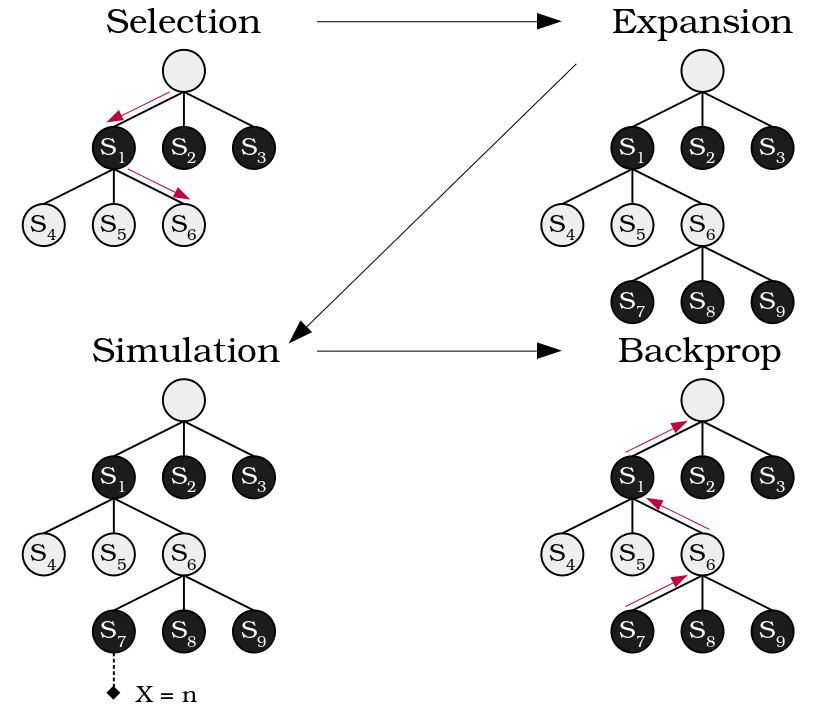
\includegraphics[width=3.5in]{fig/mctsFuncs.png}
	\caption{4 Main Steps for the Creation of a Monte Carlo Tree}
	\label{fig:mctsFunc}
\end{figure}

\subsection{Selection} 
At the start of each iteration, the program initializes at the root of the tree $id = 0$, and from its children, select the child with the highest associated UCB1 value. With $X$ being the future reward from exploring the node, $N$ being the number of visits the node has recieved, and $n$ being the number of visits the parent node has recieved. 
\begin{equation}
    \label{eq:UCB1}
    \text{UCB1 Node Value: } X + C_p \sqrt{\frac{\ln{n}}{N}}
\end{equation}

In the case of $C_p$, the exploration-exploitation parameter, a value of $C_p = \frac{1}{\sqrt{2}}$ was selected due to its performance demonstrated by Hennes \cite{Hennes2015}. This reward policy allows the tree to explore all available nodes, while still exploiting nodes that return high enough future rewards.

Once a child node has been selected, this process will repeat until a leaf node, a node with no children, has been reached. As the function navigates down a branch, the string of nodes leading to a leaf, if all of a selected nodes children are deemed terminal, such as exceeding the total $\Delta V$ budget, the current node is also declared terminal. When this condition is met, the select function will restart its search process at root of the tree. With this implementation, the tree is able to further constrict the search space, reducing computation time. Once the selection process leads to a leaf node, the node $id$ will be passed to the expansion function for the next step of building the tree. %As the branch, the string of nodes leading to a leaf, is being explored, the function also evaluates the all children of each node for is they lead to a terminal condition, such as running out of the fuel budget. If all child nodes are considered terminal, then the associated parent node is also considered terminal, and the function restarts at the top of the tree. This process was implemented in order to prune the tree of any branches that showed results initially, but lead to all terminal states. Once the function has reached a leaf node, it will return the id associated and move onto the next step in building the tree, expansion.

\subsection{Expansion}
Before the creation of the new set of nodes, the function will first look at the state of the current node being expanded from as a base. As planetary motion is one of conic sections, cartesian grid position sampling is not viable, thus angular divisions are required to efficiently sample a planets position. For each of the possible planets to visit, the following policy will be implemented. 

\begin{equation}
    \label{eq:ephemArray}
    E = 
    \left(\begin{array}{c}
        n*(\tau_1 + \tau_0) + t_0 \\ 
        \vdots \\
        m*(\tau_1 + \tau_0) + t_0 \\
    \end{array}\right)
    \text{ for } 
    \left\{\begin{array}{lll} 
        n = 0.1, & m = 1.0 &\text{if } a_1 < 2 \text{ AU} \\ 
        n = 0.05, & m = 0.25 &\text{if } a_1 \geq 2 \text{ AU}
    \end{array}\right.
\end{equation}

For the ephemeris time array $E$, the ephemeris time of the child node is dictated by the period child node's planet, $\tau_1$, and the period of the parent node's planet, $\tau_0$. This array is bounded using the parameters $n$ and $m$, which are defined by the semi-major axis of the child node's planet, $a_1$. The values for $n$ and $m$ for the inner planets, $a_1 < 2$ AU, were selected upon their performance in Hennes \cite{Hennes2015}. These values were not ideal for travel to the outer planets, as it lead to Lambert arc time of flights in excess of 12 years for travel to Jupiter. Additionally, if Jupiter were to be used for a graviational assist to another outer body, faster transfers were required. Based on their performance in simulations, the values of $n = 0.05$ and $m = 0.25$ lead to more transfers that satisified mission requirements. %determined based on the performance of the tree, for outer planet destinations, early, faster arrivals were prefered, so their parameters have been reduced to reflect as such. 

With the upper and lower bounds of the array set, an additional parameter, defined by the user, $d$ specifies the length of the array, also defining the resolution of the time steps. Additionally, this allowed for dynamic angular detail in the ephemeris time arrays. The inner planetary sequences are more sensitive to small time disturbances, and could lead to missed transfers. Thus, the fixed array length made the time steps smaller for inner planets, and coarser for the outer planets, which were much less sensitive to the time differences of each node. For the purpose of this paper, a value of $d = 16$ was found to be sufficient for all calculations as a balance between computation time and detail. 

Furthermore, children nodes that revisit the same parent planet have additional epheremis node tweaks to allow for better performance. $n$ and $m$ have their values set to 0.9, and 1 accordingly, for the set values in $k$. This allows the tree to search differing, non-impulsive, leveraging orbits of 2:1, 3:1, and 4:1 resonances. At this time, only leveraging sequences with revolutions of less than 1 were allowed.

\begin{equation}
    \label{eq:ephemArrayLev}
    E = 
    \left(\begin{array}{c}
        k*n*\tau + t_0 \\ 
        \vdots \\
        k*m*\tau + t_0 - 3 \text{ days} \\
    \end{array}\right)\hspace{1.5em}
    \text{For } k \text{ in } [2, 3, 4]
\end{equation}

Once the list of states has been established, a new set of children nodes are created to match all combinations of ephemeris times and planetary NAIF ID pairs. In order to further prune the tree to reduce unnecessary calculations, Lambert arcs are calculated to each state pair to evauluate their associated $\Delta V$ cost. Any node that exceeds the mission budget is considered terminal and not used in any further exploration. In order to calculate mission $\Delta V$ usage, the simulation uses powered flybys, as characterized by Wagner \cite{Wagner2015}.

The powered flyby geometry consists of an incoming and outgoing spacecraft velocity vectors given by the solutions to the Lambert’s problem. This maneuver is used to either torque the spacecraft to a desired direction and/or further increase/decrease the magnitude of $V_{\infty, out}$. Therefore, a small $\Delta V$ investment is used in order to increase the performance and efficiency of the gravity assists. This maneuver can be performed at any location along the incoming and outgoing velocity vectors. Its effectiveness, moreover, is derived from the Oberth effect, which states that a $\Delta V$ maneuver is more efficient to change the overall orbital energy at high velocities. For this reason, it is common to design the maneuver at periapsis \cite{Brennan2015}. 

From this we can arrive at the formulation from Wagner as a Boundary Value Problem (BVP)\cite{Wagner2015}. It can be assumed that the flyby is coplanar, and the plane can be defined by the incoming and outgoing spacecraft velocities and the center of the encounter planet. The conditions that define the BVP are the incoming and outgoing $V_\infty$ and the total turning angle, $\delta$. The solution to the BVP is the $\Delta V$ and the value of the maneuver periapsis radius, $r_p$. The first initial condition to the problem is the semimajor axis, $a$, of the incoming and outgoing hyperbolic trajectories which is defined as:

\begin{equation}
    a_\text{in/out} = -\frac{\mu_p}{v^2_{\infty-\text{in/out}}}
\end{equation}

Where $\mu$ is the gravitational parameter of the flyby planet. Additionally, the required turn angle from the flyby, $\delta$, is another condition that must be met. This value is found by the following function finding the angle between the incoming and outgoing $V_\infty$ vectors:

\begin{equation}
    \delta = \text{cos}^{-1}\left(\frac{ \vec{\textbf{V}}_{\infty-\text{in}} \cdot \vec{\textbf{V}}_{\infty-\text{out}} }{ V_{\infty-\text{in}} \cdot V_{\infty-\text{out}} }\right)
\end{equation}

With $e_{out}$ as the iterated value, a function, and its derivative, can be defined. Using the Newton Raphson method of root finding to solve for the $e_{out}$ that coinsides with the two $V_\infty$ vectors. For each full loop, an initial $e_{out}$ value of 1.5 is used due to its performance in Wagner \cite{Wagner2015}.

\begin{equation}
    f = \left( \frac{a_{out}}{a_{in}} (e_{out} - 1) \right) \text{sin} \left( \delta - \text{sin}^{-1} \left( \frac{1}{e_{out}} \right) \right) 
\end{equation}

\begin{equation}
    \frac{\text{d}f}{\text{d}e_{out}} = \left( \frac{a_{out}}{a_{in}}e_{out} - a_{out}{a_{in}} + 1 \right) \frac{ \text{cos}\left( \delta - \text{sin}^{-1} \left( \sfrac{1}{e_{out}} \right) \right) }{ e_{out}^{2} \sqrt{1 - \sfrac{1}{e_{out}^{2}} } } + \frac{a_{out}}{a_{in}}\text{cos}\left( \delta - \text{sin}^{-1} \left( \sfrac{1}{e_{out}} \right) \right)
\end{equation}

Once a value of $e_{out}$ has been found, it can then be used to find the actual periapsis radius, which is then used to find the required $\Delta V$. In addition, the periapsis radius is checked again body radius to prevent solutions that impact the planet's surface. 

\begin{equation}
    r_p = a_{out}(1 - e_{out})
\end{equation}

\begin{equation}
    \Delta V_{GA} = \left| \sqrt{ v^2_{\infty-\text{in}} + \frac{2\mu}{r_p} } - \sqrt{ v^2_{\infty-\text{out}} + \frac{2\mu}{r_p} } \right|
\end{equation}

While this results in an increased computation cost at each step of the node creation process, this method of $\Delta V$ calculation allows for a better approximation of real life trajectory performance. In addition to powered flyby $\Delta V$'s, fuel usage was also calculated for launch energies higher than the specified limit. If that max launch energy was defined as C3 = 36 $\sfrac{km^2}{s^2}$ and the spacecraft launched at a $V_\infty$ = 7 $\sfrac{km}{s}$, the incurred $\Delta V$ cost would be 1 $\sfrac{km}{s}$. 

After the states have been created, and the nodes pruned, the expand function selects the new node with the lowest associated $\Delta V$ cost to continue onto the Simulation step.

\subsection{Simulation}

On the tree's arrival to an unvisited leaf node, the node's future expected reward, $X$, must be calculated. A group of temporary state pairs are expanded from the leaf, as starting point for the random exploration. For each new node, the program will randomly walk through additional state pairs, generated in the same fashion as in the expand function, calculating the $\Delta V$ in the process, until a termination state is reached. When either the budget is expended or the target planet is reached, the associated cost is calculated using the equations below.

\begin{equation}
    \label{eq:simCost1}
    X = \text{max}\left( 0.1 \cdot l,\hspace{0.5em} \frac{\Delta V_{budget} - \Delta V_{used}}{\Delta V_{budget}} \right)
\end{equation}

Upon termination, the reward is balanced between two criteria: $\Delta V$ usage, and number of flybys completed, $l$. In the case were the final desination is not reached within the allowed budget, the algorithm will still provide a small benefit to a simulation completing Lambert arcs. After all temporary states have been simulated from, the reward returned from each is averaged and output from the function to be passed back up the branch.

\subsection{Backpropagation}

At the end of the core MCTS loop, the backpropagation step communicates the expected reward from a leaf node back up the branch to reflect a more accurate reward of a branch. The $X$ of each node in the branch is adjusted based of a weighted average of its previously observed rewards. 

\begin{equation}
    \label{eq:bp}
    X_{node, new} = \frac{X_{node, old} \cdot N_{node} + X_{new}}{N_{node} + 1}
\end{equation}

Once the cost is propagated up the tree, the loop restarts at another iteration, exploring a new set of state pairs. This process will repeat until the computation budget is depleted. At completion, the tree will evaluate all leaf nodes that meet the mission constraints to passed to the next step in the trajectory design process, optimization.

\section{$\boldsymbol{\Delta V}$EGA Maneuver Implementation}

A $\Delta V$EGA orbit, also referred to as a leveraging orbit specifically of Earth, launches with the intent to gravity assist off the body for a higher post-flyby heliocentric energy\cite{Hollenbeck}.  Leveraging orbits are classified by their nominal resonance period multiple with respect to the flyby body's heliocentric orbit, and we will refer to this number as "$k$." For example, a leveraging orbit that has a period roughly 3 times as large as Earth's will have a $k=3$ which is represented as a 3:1 $\Delta V$EGA trajectory. The actual period of these orbits will vary either greater than or less than the nominal time due to flying by the body at a different Earth heliocentric true anomaly. Trajectories with a larger period are referred to as $k$:$1^{+} \Delta$VEGA and those with a shorter are $k$:$1^{-} \Delta$VEGA trajectories. To modify the flyby Earth true anomaly a maneuver at the aphelion (deep space maneuver) is executed.

The deep space maneuver (DSM) and subsequent Earth launch characteristics are calculated before the tree generation in order to reduce the required number of computations within the search. We approximate the $\Delta$V requirements for both maneuvers, and their inclusion reduces the discontinuous trajectory endpoint velocities needed to patch Earth-Earth flyby sequences. Having the required aphelion $\Delta$V can also aid the optimization process initial guess. A lookup table sorted by the nominal resonance multiple ($k$) and encounter true anomalies ($\theta_{E}$) contains the resulting leveraging orbit properties and maneuver magnitudes. Due to being a rough approximation, the circular Earth orbit and coplanar trajectories assumptions are used. Finding the $\Delta V$EGA orbit parameters for a specific encounter true anomaly ($\theta_{E}$) and $k$ begins by assuming a nominal orbit period launch and its associated $V_\infty$. The state elements are computed at Earth and the resulting aphelion radius and velocity are found. Because the intercept true anomaly is fixed, its location and the time it takes to reach the point are known. Eq.~\eqref{eq:dteqn} is the difference in time from the DSM maneuver location to the Earth gravity assist (EGA) point where $T_E$ is the orbital period of Earth.

\begin{equation}
	\label{eq:dteqn}
	dt = kT_E \pm T_E(\theta_E/2\pi)
\end{equation}


\begin{figure}[htb]
	\centering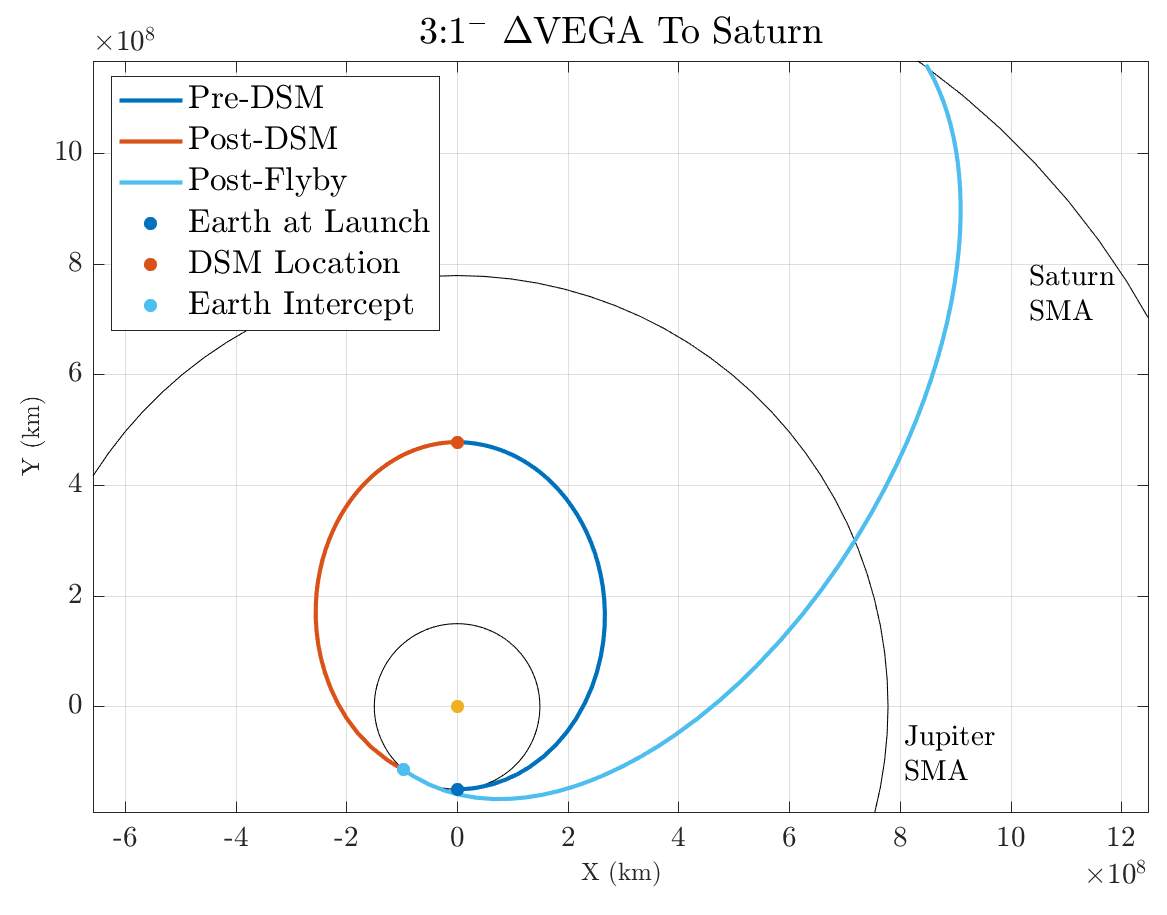
\includegraphics[width=3.6in]{./fig/dsmmatlab}
	\caption{Example of a computed 3:$1^{-} \Delta$VEGA trajectory to Saturn's semi-major axis. The launch $V_\infty$ is 6.97 km/s and the required DSM $\Delta$V is 0.39 km/s. The EGA flyby altitude was constrained to 200 km, which yielded the highest post flyby energy.}
	\label{fig:dsmmatlab}
\end{figure}

A Lambert arc is computed between these points and the resulting initial velocity change is used to find the DSM vector. The final velocity vector is assumed to be the heliocentric velocity of the leveraging orbit at the EGA. The relative velocity, $\vec{V_\infty}$ is computed and a planar flyby of Earth can now be calculated from the tree search algorithm. Fig.~\ref{fig:dsmmatlab} illustrates an example leveraging orbit being calculated for $\theta_{E}$ = 40.$7^{\circ}$. An energy maximizing flyby and propagation to the new aphelion is added to the end of the $\Delta V$EGA orbit to show the resulting trajectory.

From testing, we noticed that as $\mid\theta_E\mid$ increased, a normal component of the DSM $\Delta$V appeared and grew larger. To limit the $\Delta$V to only a tangential component, and in return to reduce the total $\Delta$V required, a minimizer can be employed. This optimization comes at the expense of a higher launch energy and a longer flight time for trajectories requiring large $\mid\theta_E\mid$. Differing trends from Sims et. al. analysis of $V_\infty$ leveraging\cite{sims1994} were only noticed in high total $\Delta$V cases for each $k$ leveraging orbit family. These solutions were discarded from the lookup table due to delivering lower aphelion radii post-flyby when compared to lower total $\Delta$V leveraging orbits of the same family. The case presented in Fig.~\ref{fig:dsmmatlab} is intended to matche that discussed by Sims et. al\cite{Sims1997} and has nearly identical results. The inclusion of deep space maneuvers, not specific to $\Delta V$EGAs, are not implemented in the current form of the tree search. However, because the algorithm patches the two conics forming the leveraging orbit using the Lambert's method, the possibility to extend DSM maneuvers for off-tangent $V_\infty$ departures and targeting for the flyby can be implemented. This inclusion adds another dimension to the lookup table but offers leveraging maneuvers between Earth and Venus.

Now that the $\Delta V$EGA orbit properties are known, the lookup table solution can be extended to the actual solar system model in the tree search. The table values are represented in a relative frame with respect to Earth's state vector at the launch epoch. A subsequent transformation of the departure velocity and pre-EGA incoming $\vec{V_\infty}$ can be done in order to find their specific components corresponding to an Earth epoch in the Ecliptic J2000 frame. From the initial node in the tree, a set of Earth leveraging time-of-flight nodes are created corresponding to their respective $k$ and $\theta_E$ parameters. The number of these leveraging nodes included in the initial flight time layer of the tree is directly related to the angular spacing of $\theta_E$. As the resolution becomes finer, by increasing the $\textit{detail}$ input to the search, the estimated $\Delta$V becomes more accurate. This, however, increases of the number of tree nodes created, and so for a rough idea of the trajectory search space, a coarse resolution is preferred. The discontinuous $\Delta$V post-EGA required to patch the incoming leg from the leveraging orbit and outgoing leg to the next planet node will determine if the leveraging node and its performance is effective for the transfer. Using this method, a distinction between the $\Delta V$EGA trajectory families to different outer planets can be observed.

\section{Performance Evaluation}

As this program was developed with no basis for its astrodynamics, multiple studies on the validation of the methods were conducted. Three major cases were explored to highlight the different core functionalities of the algorithm. The first case is a search to find Europa Clippers non-SLS trajectory involving a sequence of 4 planetary flyby's, to test MCTS's ability to find long sequence trajectories. The second study is designed to push the limits of powered flyby $\Delta V$ theory, by finding Galileo's low budget trajectory to Jupiter with similar efficiency. The final case is not based off any historical mission, but built to test the flexibility of the $\Delta V$EGA theory by finding a variety of the launch possibilities for a Trident-like mission to Neptune.

In addition to matching results found in currently published research, each case will forward their inputs to MALTO (Mission Analysis Low Thrust Optimizer). While this software is primarily built for low-thrust applications, the program is still capable of taking inputs for ballistic and chemical propulsion trajectories \cite{Sims2006}. For each leg of the mission, the optimizer was allowed $\pm$ 100 days on either side of MCTS's intial guess to mitigate the coarse nature of the broad searches constraints. 

\subsection{Case 1: Europa Clipper Trajectory Recreation}

For the first case, a search was conducted of Europa Clipper's launch window. The goal in mind was to find the EEVEEJ trajectory, as shown by Buffington\cite{Buffington2014}. The nominal trajectory has the spacecraft set to launch on June 03, 2022, and arriving at Jupiter on January 15, 2030 with an additional 3 Earth flybys and 1 Venus flyby. The primary challenge for this mission was the complexity of the sequence, as the difficulty of the combinational problem grows non-linearly with length.
\begin{table}[htb]
    \centering
    \caption{Constrain Input Table for Europa Clipper Trajectory Search}
    \label{table:clipInputs}
    \begin{tabular}{lc}
        \toprule
        \textbf{Input Name} & \textbf{Input Value}\\
        \midrule
        Arrival Planet & Jupiter \\
        Launch Window & March 01, 2022 --- September 01, 2022 \\
        Iterations & 75,000 \\ 
        $\Delta V$ Budget & 10 $km/s$ \\
        Max C3 & 10 $km^2/s^2$ \\
        Detail ($d$) & 24 \\
        \bottomrule
    \end{tabular}
\end{table}


Table \ref*{table:clipInputs} provides the search criteria for the broad trajectory search. For general trajectory searches, it was found that an iteration budget of 50,000 was found to be sufficient for most trajectories, but due to the length of the planetary sequence for the nominal trajectory, the iteration limit had to be adjusted. Runs with a $d = 16$ were also conducted, but due to the coarseness in the separation of state pairs, the exact solution was deemed infeasible. As described earlier, this behavior is one of the drawbacks of heuristic searches as not all possible solutions can be found. 

At the completion of the search, the algorithm had conducted 20 million Lambert arcs, and created one million tree nodes. Of the 1.9 billion possible combinations possible for a 6 layer tree, only 275 solutions were deemed feasible for the input criteria. Figure \ref*{fig:clipResults} (Left) shows the top 100 trajectories, sorted by their unoptimized mission $\Delta V$ with the nominal circled and shown on the (Right). The targeted sequence was the ninth highest result in terms of unoptimized $\Delta V$ usage behind an EEVVEJ and EEVEJ sequence. The trajectories non-podium finish is down to the final Earth flyby, which even under ideal dates requires a flyby $\Delta V$ of 3.23 $\sfrac{\text{km}}{\text{s}}$. Among all top performing trajectories, the initial two flybys of Earth and Venus were held in common sharing similar dates. Of the EEVEEJ solutions found, the most optimal utilized a 3:1 orbital resonance for the final Earth flyby, while the nominal trajectory utilized a 2:1. The 2:1 solutions also exist within the results, but do not appear until later is the data set, utilizing an additional 250 $\sfrac{\text{m}}{\text{s}}$ of $\Delta V$. Even with this deviation, the Jupiter arrival occured only one month later than targeted and with a lower incoming $V_\infty$.


\begin{figure}[htb]
    \begin{subfigure}
        \centering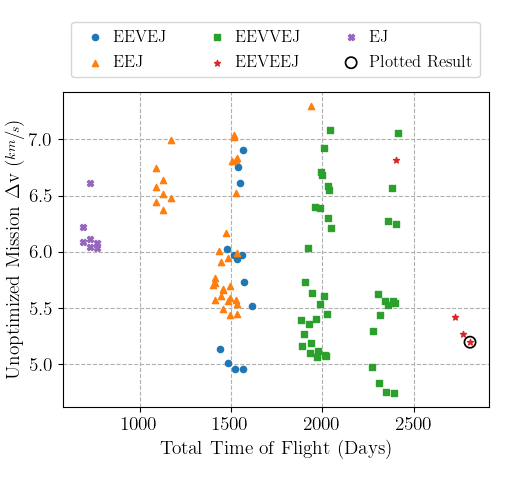
\includegraphics[width=2.75in]{./fig/clipperResults.png}
    \end{subfigure}
    \begin{subfigure}
        \centering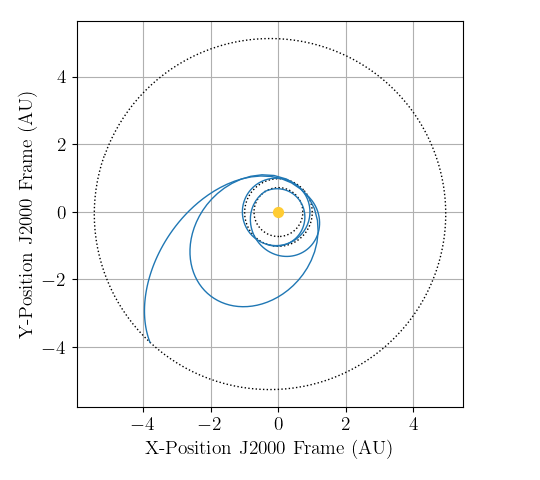
\includegraphics[width=3in]{./fig/clipperMCTS.png}
    \end{subfigure}
    \caption{(Left) Top 100 results from built broad search colored by sequence\hspace{1em} (Right) Circled, unoptimized trajectory from results that matches targeted sequence from Buffington \cite{Buffington2014}}
    \label{fig:clipResults}
\end{figure}

Utilizing the highest performing EEVEEJ transfer, the dates MCTS supplied were optimized using MALTO. Table \ref*{table:clipMInputs} shows initial guess supplied to MALTO by MCTS as well as the post optimized dates that MALTO returned. To allow the minimization of the arrival $V_\infty$, the date bounds for Jupiter were adjusted to be $\pm$ 500 days. 

Upon completion the optimization run, MALTO had converged on the solution in Figure \ref*{fig:clipMalto}. The resulting trajectory was well within the bounds placed on the optimizer for the flybys and arrival dates, as well, the arrival $V_\infty$ was reduced. In addition, the largest departure from the intial guess dates from MCTS, apart from Jupiter arrival, was the third flyby of Earth. The date had transitioned 1.5 months later than initially chosen, leading to an orbit of more than 1 complete revolution. With this test complete, it can be shown that this MCTS algorithm is capable in searching out long sequence interplanetary trajectories that need minimal tweaking in later steps of the optimization process. % The results fall well within the 100 day bounds set on the program, with the greatest change, in terms of dates, being the later Jupiter arrival and the last Earth flyby occuring 1.5 months later. Even though the unoptimized $\Delta V$ was well above 5 $\sfrac{km}{s}$, the optimized solution was able to entirely eliminate any $\Delta V$ cost. 

\begin{figure}[tb]
    \centering
    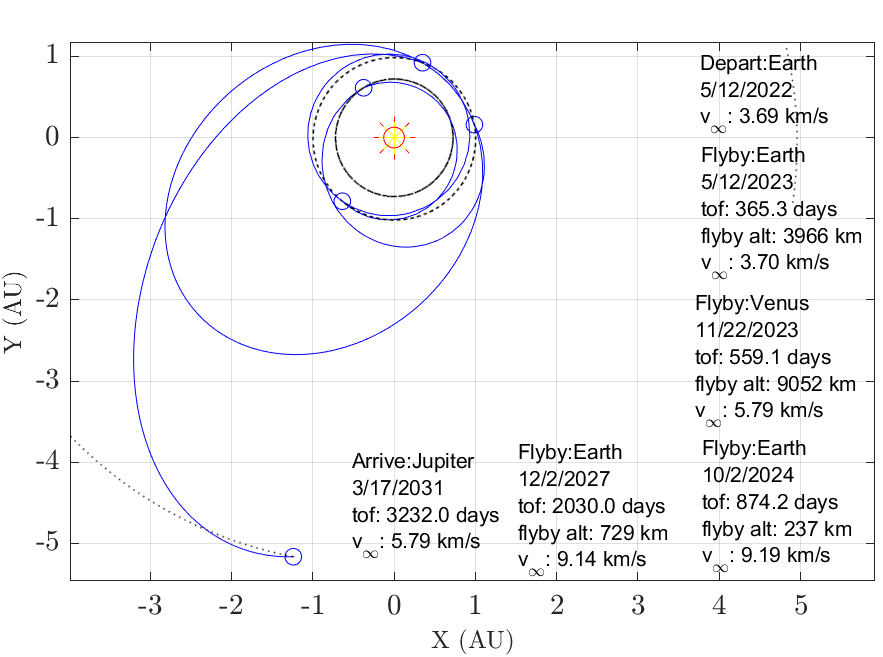
\includegraphics[width = 5in]{./fig/clipperMalto.png}
    \caption{MALTO optimized Europa Clipper trajectory from MCTS dates}
    \label{fig:clipMalto}
\end{figure}

% \iffalse
\begin{table}[htb]
    \begin{center}
        \caption{MCTS output dates vs MALTO optimized dates}
        \label{table:clipMInputs}
        \begin{tabular}{lcc}
            \toprule
            \multirow{2}{*}{\textbf{Planetary Node}} & \multicolumn{2}{c}{\textbf{Dates}}\\
            \cmidrule{2-3}
            {} & \textbf{MCTS} & \textbf{MALTO}\\
            \midrule
            Launch & June 04, 2022 & May 12, 2022 \\
            Earth Flyby \#1 & Jun 02, 2023 & May 12, 2023 \\
            Venus Flyby & November 23, 2023 & November 22, 2023 \\ 
            Earth Flyby \#2 & October 22, 2024 & October 2, 2024 \\
            Earth Flyby \#3 & October 20, 2027 & December 2, 2027 \\
            Jupiter Arrival & February 13, 2030 & March 17, 2031 \\
            \bottomrule
        \end{tabular}
    \end{center}
\end{table}
% \fi

\subsection{Case 2: Galileo Trajectory Recreation}

For the second validation case, the nominal trajectory of Galileo has the spacecraft set to launch from Earth with a C3 of 13-17 $\sfrac{\text{km}^2}{\text{s}^2}$ on October 18, 1989, and arriving at Jupiter on December 07, 1995 with a Venus flyby and a Earth 2:1 resonance sequence. The major challenge behind this sequence was for MCTS to be able to find the low required $\Delta V$ solution as described by D'Amario\cite{DAmario1992}. For Galileo's interplanetary leg of its trajectory design, the spacecraft was only budgeted 100 $\sfrac{\text{m}}{\text{s}} \text{ of } \Delta V$ for TCMs, trajectory correction maneuvers. 

\begin{table}[htb]
    \centering
    \caption{Constrain Input Table for Galileo Trajectory Search}
    \label{table:galiInputs}
    \begin{tabular}{lc}
        \toprule
        \textbf{Input Name} & \textbf{Input Value}\\
        \midrule
        Arrival Planet & Jupiter \\
        Launch Window & Jun 01, 1989 --- Dec 31, 1989 \\
        Iterations & 50,000 \\ 
        $\Delta V$ Budget & 3 $\sfrac{km}{s}$ \\
        Max Arrival $V_{\infty}$ & 7.5 $\sfrac{km}{s}$  \\
        Max C3 & 20 $\sfrac{km^2}{s^2}$ \\
        Detail ($d$) & 16 \\
        \bottomrule
    \end{tabular}
\end{table}

Table \ref*{table:galiInputs} lays out the inputs to the search algorithm, which fall more in line with the average use case. In order to constrain the solution to the low $\Delta V$ solution, the $\Delta V$ budget was set to 3 $\sfrac{km}{s}$, and the maximum C3 was rounded to a value of 20 $\sfrac{km^2}{s^2}$. An additional constrain was also placed on the search, requiring a low energy arrival to Jupiter, to once again constrain the solution to that of Galileo. As a silent constraint for all searches, solutions will also be required to have a radially $V_\infty$ greater than -3 $\sfrac{km}{s}$ or less than +3 $\sfrac{km}{s}$ for radial in and out arrivals accordingly. This was implemented so that solutions contained the correct arrival $V_\infty$ direction, as well as value were found.

\begin{figure}[htb]
    \begin{subfigure}
        \centering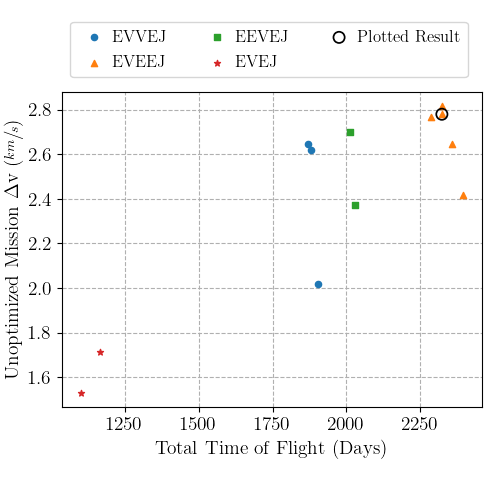
\includegraphics[width=2.75in]{./fig/galileoResults.png}
    \end{subfigure}
    \begin{subfigure}
        \centering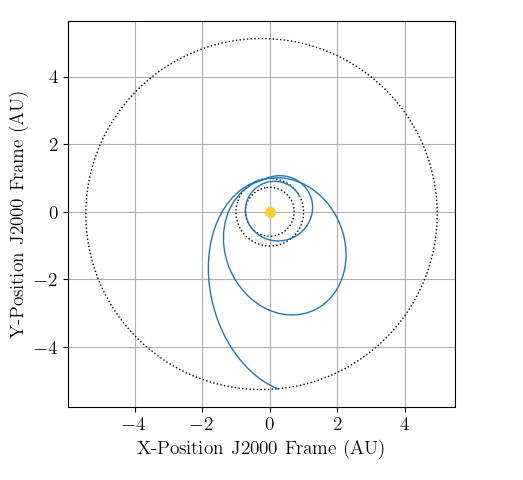
\includegraphics[width=3in]{./fig/galileoMCTS.png}
    \end{subfigure}
    \caption{(Left) Top results from built broad search colored by sequence\hspace{1em} (Right) Circled, unoptimized trajectory from results that matches targeted sequence from D'Amario \cite{DAmario1992}}
    \label{fig:galiResults}
\end{figure}

At the conclusion of the search, the tree made 867,000 nodes and conducted 10 million Lambert arcs, in order to find the 12 solutions to the constraints. Of those solutions, the eighth was the nominal targeted trajectory. Figure \ref*{fig:galiResults} (Left) shows the 12 solutions ranked by their unoptimized mission $\Delta V$ usage, and the (Right) shows the circled nominal trajectory. In the same fashion as the Europa Clipper case, the optimal found trajectory deviates from what Galileo originally performed. The final Earth flyby was conducted in a 3:1 resonance rather than a 2:1 resonance and lead to an overall smaller incoming $V_\infty$. The 2:1 resonance case also exists within the found data set, but is the 11 of 12 that satisfies the criteria. Once again, similar to Europa Clipper, with the additional 1 year resonance, the spacecraft only arrives at Jupiter 3 months after targeted. With the trajectory leg dates, this solution will be optimized using MALTO to find the optimized version of this trajectory. 

When inputting trajectory dates into MALTO, it was found the 3:1 sequence suggested was not as viable compared to other options. When converging the trajectory, it was found that the performance of the 3:1 trajectory was too high for MALTO to properly capture at Jupiter. Thus by increasing the bounds of the final Earth flyby to bounds of $\pm$500 days to give more leeway, MALTO converged on a solution that utilized a 2:1 orbit as opposed to the 3:1. This result can be found in Figure \ref*{fig:galiMalto}. This result aligns with the findings by Sims \cite{sims1994} where 3:1 orbits were capable of reaching aphelion heights of Uranus SMA, while 2:1 trajectories can reach aphelion heights of 8 AU. Doing so allowed, the work of the Jupiter transfer to be shared between the two Earth flybys without exceeding their energy capacities. As in Table \ref*{table:galiMInputs}, even after taking a year off the total flight time to the last Earth flyby, the Jupiter arrival was only set back 113 days. 

\begin{figure}[h!]
    \centering
    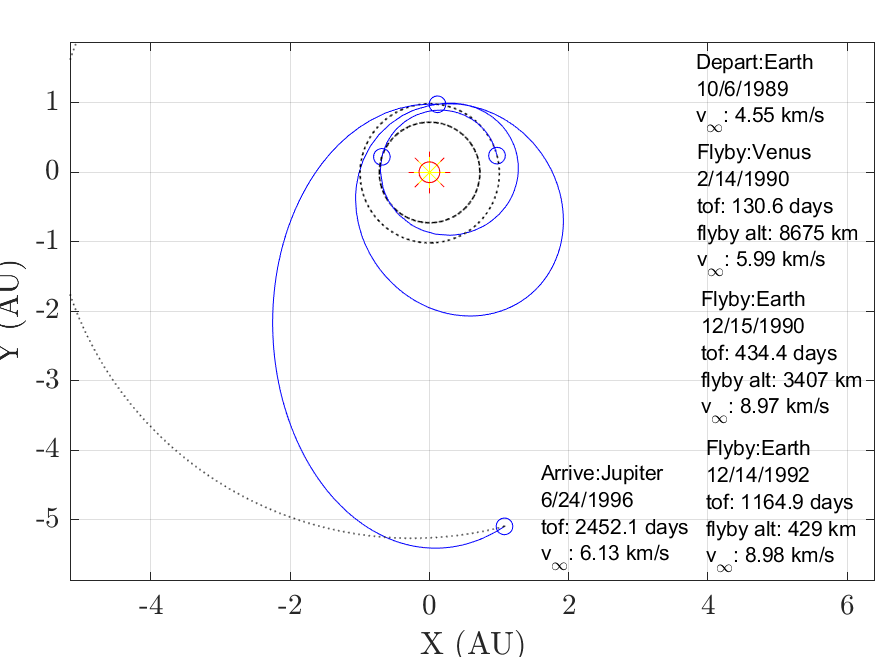
\includegraphics[width = 5in]{./fig/galileoMalto.png}
    \caption{MALTO optimized Galileo trajectory from MCTS dates}
    \label{fig:galiMalto}
\end{figure}

\begin{table}[h!]
    \begin{center}
        \caption{MCTS output dates vs MALTO optimized dates}
        \label{table:galiMInputs}
        \begin{tabular}{lcc}
            \toprule
            \multirow{2}{*}{\textbf{Planetary Node}} & \multicolumn{2}{c}{\textbf{Dates}}\\
            \cmidrule{2-3}
            {} & \textbf{MCTS} & \textbf{MALTO}\\
            \midrule
            Launch          & October 21, 1989  & October 06, 1989\\
            Venus Flyby     & February 27, 1990 & February 14, 1990 \\ 
            Earth Flyby \#1 & December 29, 1990 & December 15, 1990 \\
            Earth Flyby \#2 & December 26, 1993 & December 14, 1992 \\
            Jupiter Arrival & March 03, 1996    & June 24, 1996 \\
            \bottomrule
        \end{tabular}
    \end{center}
\end{table}
%%%%%%TEMP%%%%%%%%%
\newpage
%%%%%%%%%%%%%%%%%%%
\subsection{Case 3: Triton $\Delta V$EGA Opportunity Search}
The tree search algorithm can now be extended to an exploratory context to find possible trajectories for future concepts. With the interest in icy moon exploration in the solar system, a sequence to Neptune, and in return Triton, is explored\cite{Hubbard2010}. An arbitrary launch period was selected for this evaluation. The search is limited to trajectories with the inclusion of a $\Delta V$EGAs to evaluate its integration and performance. The number of iterations was set at 10,000 as this is seen to have a good compromise between calculation time and the number of search results. For a sequence to Neptune, it is desired to have a higher incoming relative velocity at Jupiter in order to have the appropriate outgoing energy to reach Neptune. With this in mind, the intent of the search was to find $\Delta V$EGA trajectories that deliver a high post EGA semi-major axis. The $\textit{detail}$ option is set to 16 which creates 8 $k$:1$^{-}$ and 8 $k$:1$^{+}$ nodes for each $k$ family. This spread is seen to balance the computation time (because of the number of nodes created) and the accuracy of the  DMS $\Delta$V. The C3 is set to emphasize the use of 2:1 $\Delta V$EGAs and the 3 and 4 $k$ leveraging families  would include the additional required velocity in the unoptimized $\Delta$V. The angular dispersion was set to 22 degrees yielding a fairly dense search space solution set. The results of the input search space are summarized in Table~\ref{tab:tritonInputs}:
%
%
\begin{table}[h]
    \begin{center}
        \caption{Inputs for $\Delta V$EGA Trajectories to Neptune via Jupiter}
        \label{tab:tritonInputs}
        \begin{tabular}{lc}
            \toprule
            \textbf{Input Name} & \textbf{Input Value}\\
            \midrule
            Arrival Planet & Neptune \\
            Launch Window \quad \quad & Jan 01, 2029 --- Jul 01, 2029 \\
            Iterations & 10,000 \\
            $\Delta V$ Budget & 4.5 $\sfrac{km}{s}$ \\
            Max C3 & 35 $\sfrac{km^2}{s^2}$ \\
            Detail ($d$) & 16 \\
            \bottomrule
        \end{tabular}
    \end{center}
\end{table}
%
%

The search completed in 700 seconds and resulted in 1714 sequences from the 178,545 nodes created. As expected, most solutions used the 2:1 or 3:1 leveraging maneuvers, and a few 4:1 and direct EJN sequences were found with large unoptimized $\Delta$Vs.
\textbf{Need to finish discussion on the search results.}
Fig.~\ref{fig:maltotriton} shows two optimized trajectories resulting from the search. The left plot is an example of a 2:1$^{+}$ $\Delta V$EGA which requires a launch $V_\infty$ magnitude of 5.39 $km/s$.
\textbf{Need to finish discussion on MALTO plot below.}
%
%
\begin{figure}[ht]
		\centering
		\begin{minipage}{0.50\textwidth}
				\centering
				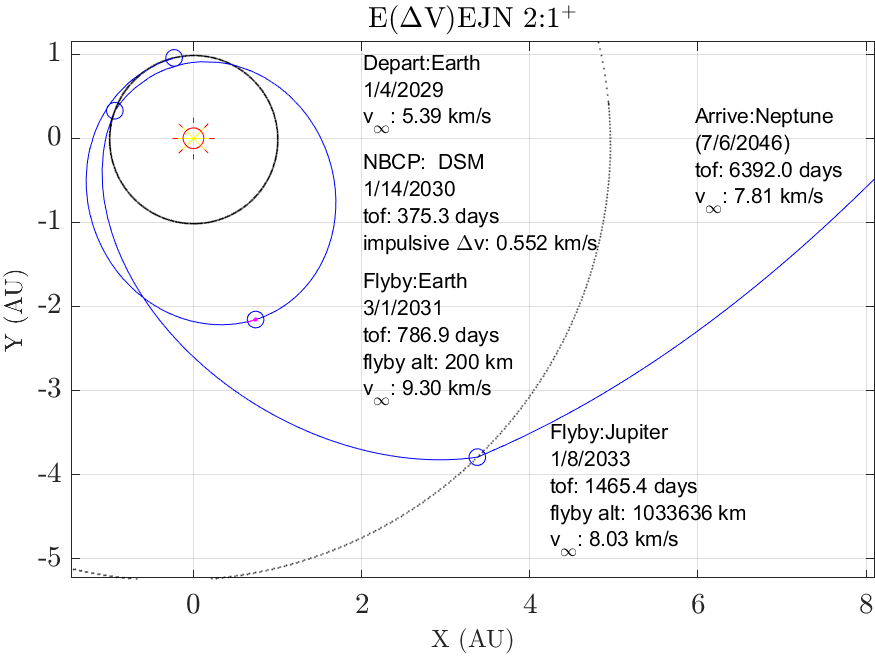
\includegraphics[width=1.0\textwidth]{./fig/eejn21plus}
    \end{minipage}\hfill
		\begin{minipage}{0.50\textwidth}
				\centering
				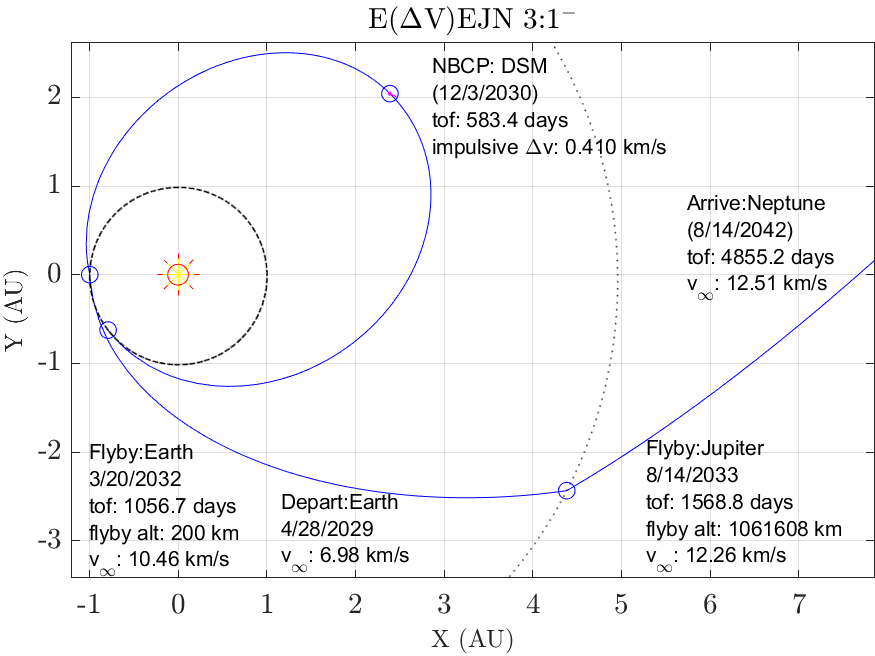
\includegraphics[width=1.0\textwidth]{./fig/eejn31minus}
		\end{minipage}
		\caption{Optimized trajectory examples from the search. The left plot is an example of a 2:1$^{+}$ and the right is a 3:1$^{-}$. The 2:1$^{+}$ is able to reach Neptune with a much lower $V_\infty$ due to a slower relative velocity into Jupiter when compared to the 3:1$^{-}$ sequence.}
		\label{fig:maltotriton}
\end{figure}
%
%
\textbf{Need to add discussion on leveraging performance}
The deep space maneuver magnitude and direction vary from the search results due to various factors. The optimization process takes into account the change in declination for the outgoing flyby and so depending on the transfer, an additional Z-component of velocity is added by the optimizer to target the appropriate Earth flyby B-Plane angle. Another source of discrepancy is in the maneuver location. In the lookup table, the assumption is that the deep space maneuver is conducted at the aphelion of the leveraging orbit. In practice, the maneuver can be shifted before of after by the optimizer. Table~\ref{tab:} summarizes a few optimized cases and their predicted DSM $\Delta$V versus the calculated value from the optimization process.


The search returns several cases of interest which have been optimized and shown in Fig.~\ref{fig:maltotriton1} and Fig.~\ref{fig:maltotriton2}. Sequences that utilize a 2:1$^{-}$ and 2:1$^{+}$ have the lowest launch energy, but also have fairly large deep space maneuvers. The
\textbf{THIS PART IS NOT DONE YET}

\iffalse
\begin{lstlisting}
def mcts.run():
    for _ in maxIterations:
        if all(launchNodes is terminal):
            break

        # Select Most Valuable Leaf Starting from Root
        id = select() 

        # Expand If Prevously Visited and Pick Most Valuable Child
        if node.children is None and node.visits is not 0:
            id = expand(id)

        # Randomly Explores From Selected Node To Generate Cost
        X = simulate(id) 

        # Propagates Results Up Branch
        backprop(id, X)
\end{lstlisting}
\fi

\appendix
\clearpage
\section{Appendix A: Raw MCTS Run Results}
\begin{table}[h!]
    \centering
    \caption{Top 23 results from broad search of Europa Clipper's launch window. Gray row shows nominal solution.}
    \begin{tabular}{lllllll}
        \toprule
        \textbf{\textbf{\#}}\hspace{2em} & \textbf{\textbf{Sequence}} & \textbf{Dep. Date}\footnotemark[1] & \textbf{\textbf{C3} $\boldsymbol{(\frac{km^2}{s^2})}$} & \textbf{$\boldsymbol{\Delta V_{unopt} (\frac{km}{s})}$} & \textbf{\textbf{ToF (Days) }} & \textbf{\textbf{Arr.} $\boldsymbol{V_\infty (\frac{km}{s})}$} \\
        \midrule
        1                           & EEVVEJ                     & 8190                            & 3.12                                                   & 4.75                                                    & 2392                       & 6.62                                                             \\
        2                           & EEVVEJ                     & 8190                            & 3.12                                                   & 5.07                                                    & 2019                       & 6.30                                                             \\
        3                           & EEVVEJ                     & 8190                            & 3.12                                                   & 5.08                                                    & 2013                       & 6.36                                                             \\
        4                           & EEVEJ                      & 8190                            & 3.12                                                   & 4.96                                                    & 1561                       & 6.54                                                             \\
        6                           & EEJ                        & 8279                            & 34.30                                                  & 5.54                                                    & 1533                       & 6.10                                                             \\
        5                           & EEJ                        & 8270                            & 35.83                                                  & 5.44                                                    & 1533                       & 6.15                                                             \\
        7                           & EEVVEJ                     & 8190                            & 3.12                                                   & 5.45                                                    & 2025                       & 6.27                                                             \\
        8                           & EEJ                        & 8279                            & 28.63                                                  & 5.57                                                    & 1523                       & 6.17                                                             \\
        \rowcolor{lightgray}9       & EEVEEJ                     & 8190                            & 3.12                                                   & 5.20                                                    & 2810                       & 6.58                                                             \\
        10                          & EEVVEJ                     & 8190                            & 3.12                                                   & 4.76                                                    & 2351                       & 7.02                                                             \\
        11                          & EEVVEJ                     & 8190                            & 3.12                                                   & 5.12                                                    & 1978                       & 6.71                                                             \\
        12                          & EEVVEJ                     & 8190                            & 3.12                                                   & 5.06                                                    & 1972                       & 6.76                                                             \\
        13                          & EEVEJ                      & 8190                            & 3.12                                                   & 4.96                                                    & 1520                       & 6.94                                                             \\
        14                          & EEVEJ                      & 8190                            & 3.12                                                   & 5.52                                                    & 1612                       & 6.41                                                             \\
        15                          & EEJ                        & 8270                            & 35.83                                                  & 5.44                                                    & 1492                       & 6.51                                                             \\
        16                          & EEJ                        & 8279                            & 34.30                                                  & 5.59                                                    & 1492                       & 6.45                                                             \\
        17                          & EEVVEJ                     & 8190                            & 3.12                                                   & 5.60                                                    & 2007                       & 6.45                                                             \\
        18                          & EEJ                        & 8279                            & 28.63                                                  & 5.56                                                    & 1482                       & 6.53                                                             \\
        19                          & EEVVEJ                     & 8190                            & 3.12                                                   & 5.55                                                    & 2398                       & 6.57                                                             \\
        20                          & EEVVEJ                     & 8190                            & 3.12                                                   & 5.54                                                    & 1984                       & 6.66                                                             \\
        21                          & EEVVEJ                     & 8190                            & 3.12                                                   & 5.40                                                    & 1966                       & 6.84                                                             \\
        22                          & EEVVEJ                     & 8190                            & 3.12                                                   & 5.56                                                    & 2386                       & 6.68                                                             \\
        23                          & EEVEEJ                     & 8190                            & 3.12                                                   & 5.26                                                    & 2769                       & 7.01                                                             \\ 
        \bottomrule
    \end{tabular}
\end{table}

\begin{table}[h!]
    \centering
    \caption{All results from broad search of Galileo's launch window. Gray row shows nominal solution.}
    \begin{tabular}{lllllll}
        \toprule
        \textbf{\textbf{\#}}\hspace{2em} & \textbf{\textbf{Sequence}} & \textbf{Dep. Date}\footnotemark[1] & \textbf{C3} $\boldsymbol{(\frac{km^2}{s^2})}$ & \textbf{$\boldsymbol{\Delta V_{unopt} (\frac{km}{s})}$} & \textbf{\textbf{ToF (Days) }} & \textbf{\textbf{Arr.} $\boldsymbol{V_\infty (\frac{km}{s})}$} \\ 
        \midrule
        1                           & EVEJ                       & -3739                           & 19.71                                         & 1.71                                                    & 1162                       & 6.64                                                             \\
        2                           & EVEJ                       & -3739                           & 19.71                                         & 1.53                                                    & 1099                       & 7.38                                                             \\
        3                           & EVEEJ                      & -3781                           & 20.75                                         & 2.42                                                    & 2395                       & 6.73                                                             \\
        4                           & EVVEJ                      & -3739                           & 19.71                                         & 2.02                                                    & 1904                       & 7.27                                                             \\
        5                           & EVEEJ                      & -3739                           & 15.94                                         & 2.65                                                    & 2360                       & 6.67                                                             \\
        6                           & EEVEJ                      & -3852                           & 27.93                                         & 2.37                                                    & 2030                       & 7.17                                                             \\
        7                           & EVEEJ                      & -3710                           & 28.73                                         & 2.82                                                    & 2325                       & 6.72                                                             \\
        \rowcolor{lightgray}8       & EVEEJ                      & -3724                           & 21.75                                         & 2.78                                                    & 2325                       & 6.87                                                             \\
        9                           & EEVEJ                      & -3824                           & 28.97                                         & 2.70                                                    & 2013                       & 7.09                                                             \\
        10                          & EVVEJ                      & -3710                           & 15.42                                         & 2.62                                                    & 1879                       & 7.24                                                             \\
        11                          & EVEEJ                      & -3724                           & 22.03                                         & 2.77                                                    & 2289                       & 7.20                                                             \\
        12                          & EVVEJ                      & -3710                           & 15.42                                         & 2.65                                                    & 1869                       & 7.33                                                             \\ 
        \bottomrule
    \end{tabular}
\end{table}

\begin{table}[h!]
    \centering
    \caption{Top 25 results from $\Delta V$EGA search to Neptune launch window. Gray row shows solutions optimized above.}
    \begin{tabular}{lllllll}
    \toprule
    \textbf{\#}\hspace{2em} & \textbf{Sequence} & \textbf{Dep. Date}\footnotemark[1] & \textbf{C3} $\boldsymbol{(\frac{km^2}{s^2})}$    & $\boldsymbol{\Delta V_{unopt} (\frac{km}{s})}$  & \textbf{ToF (Days)} & \textbf{Arr.} $\boldsymbol{V_\infty (\frac{km}{s})}$ \\ 
    \midrule
    \rowcolor{lightgray}1                  & E(2:1+)EJN        & 10593                 & 29.08       & 1.17        & 6385      & 7.84          \\
    2                  & E(2:1+)EJN        & 10593                 & 29.08       & 1.35        & 7240      & 6.27          \\
    3                  & E(2:1+)EJN        & 10593                 & 28.14       & 1.42        & 6371      & 7.86          \\
    4                  & E(2:1+)EJN        & 10593                 & 28.14       & 1.43        & 5516      & 10.12         \\
    5                  & E(2:1+)EJN        & 10593                 & 28.14       & 1.47        & 4598      & 13.77         \\
    6                  & E(2:1+)EJN        & 10593                 & 29.08       & 1.48        & 8095      & 5.14          \\
    7                  & E(3:1-)EJN        & 10713                 & 48.30       & 1.48        & 7385      & 6.01          \\
    8                  & E(2:1+)EJN        & 10593                 & 28.14       & 1.51        & 8999      & 4.3           \\
    9                  & E(2:1+)EJN        & 10593                 & 29.08       & 1.57        & 5530      & 10.09         \\
    10                 & E(2:1+)EJN        & 10593                 & 29.08       & 1.58        & 9012      & 4.29          \\
    11                 & E(2:1+)EJN        & 10593                 & 29.08       & 1.58        & 8950      & 4.32          \\
    12                 & E(2:1+)EJN        & 10593                 & 29.08       & 1.59        & 4612      & 13.73         \\
    13                 & E(2:1+)EJN        & 10593                 & 28.14       & 1.61        & 7226      & 6.29          \\
    14                 & E(2:1+)EJN        & 10593                 & 28.14       & 1.63        & 8144      & 5.11          \\
    15                 & E(2:1+)EJN        & 10593                 & 29.08       & 1.69        & 8157      & 5.1           \\
    16                 & E(3:1-)EJN        & 10701                 & 48.30       & 1.71        & 6530      & 7.47          \\
    17                 & E(3:1-)EJN        & 10713                 & 48.30       & 1.72        & 8240      & 4.99          \\
    18                 & E(2:1+)EJN        & 10605                 & 28.14       & 1.73        & 6371      & 7.84          \\
    19                 & E(3:1-)EJN        & 10713                 & 48.30       & 1.74        & 6530      & 7.46          \\
    20                 & E(2:1+)EJN        & 10593                 & 28.14       & 1.74        & 8081      & 5.16          \\
    21                 & E(2:1+)EJN        & 10593                 & 28.14       & 1.76        & 7289      & 6.22          \\
    22                 & E(2:1+)EJN        & 10593                 & 29.08       & 1.83        & 7302      & 6.2           \\
    23                 & E(2:1+)EJN        & 10593                 & 28.14       & 1.84        & 8936      & 4.33          \\
    24                 & E(3:1+)EJN        & 10641                 & 49.38       & 1.85        & 7457      & 6.01          \\
    \rowcolor{lightgray}25                 & E(3:1+)EJN        & 10713                 & 48.63       & 2.35        & 4752      & 12.95         \\                                                 
    \bottomrule
    \end{tabular}
\end{table}
\footnotetext[1]{Days since January 01, 2000 (J2000)}

\clearpage

\section{Appendix B: Sequence Family Plots}
\begin{figure}[h!]
    \begin{subfigure}{}
        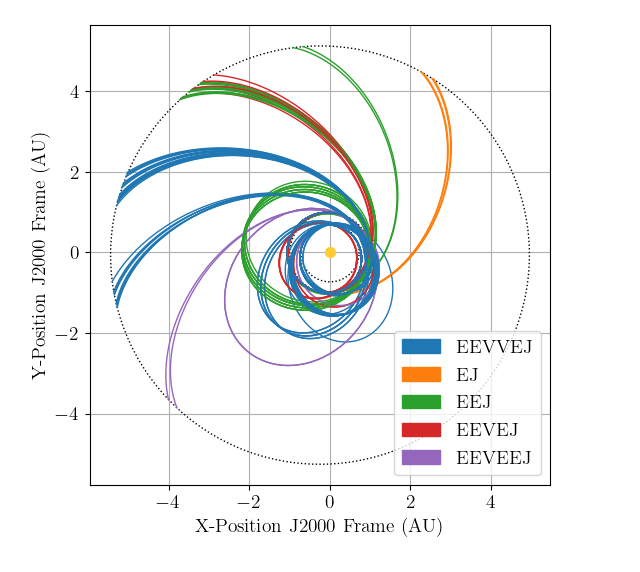
\includegraphics[width=3in]{./fig/clipperFamilies.png}
        \label{fig:clipFam}
        % \caption{Top 25 results from Europa Clipper dataset, color sorted by sequence}
    \end{subfigure}
    \begin{subfigure}{}
        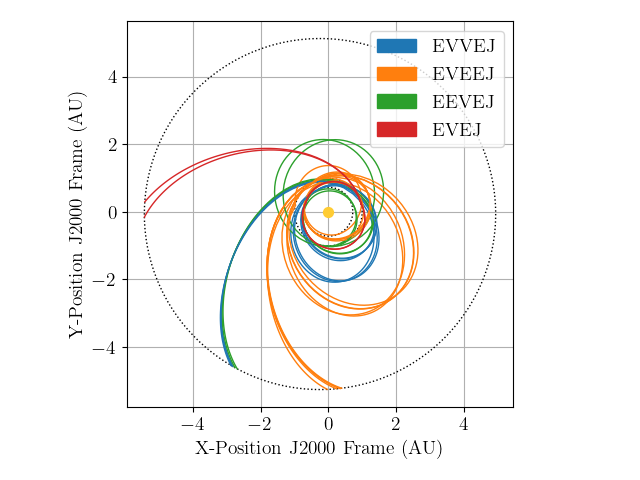
\includegraphics[width=3.55in]{./fig/galileoFamilies.png}
        \label{fig:galiFam}
        % \caption{Top 12 results from Galileo dataset, color sorted by sequence}
    \end{subfigure}
    \caption{(Left) Top 25 results from Europa Clipper dataset, color sorted by sequence (Right) Top 12 results from Galileo dataset, color sorted by sequence}
\end{figure}
\begin{figure}[h]
    \centering
    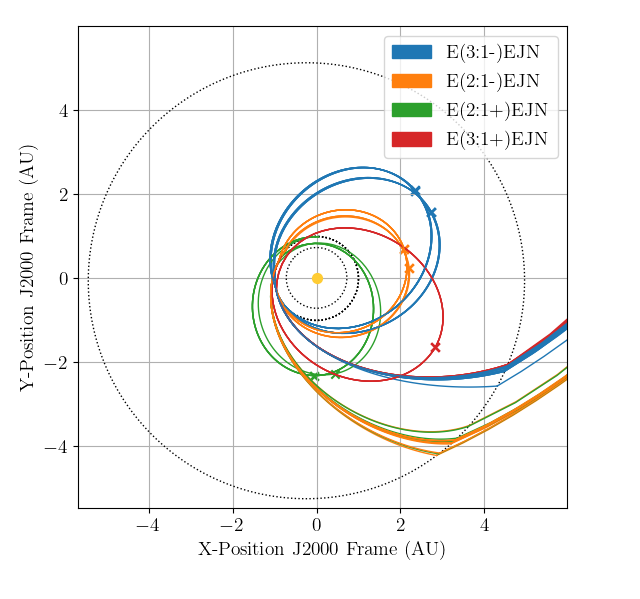
\includegraphics[width=3in]{./fig/tridentFamilies.png}
    \label{fig:tridFam}
    \caption{Top 25 results from Neptune Flyby dataset, color sorted by sequence}
\end{figure}


\clearpage
\bibliographystyle{AAS_publication}   % Number the references.
\bibliography{references}   % Use references.bib to resolve the labels.

\end{document}